% Created 2017-04-22 Sat 12:45
% Intended LaTeX compiler: pdflatex
\documentclass[10pt,aspectratio=1610]{beamer}
\usepackage[utf8]{inputenc}
\usepackage[T1]{fontenc}
\usepackage{graphicx}
\usepackage{grffile}
\usepackage{longtable}
\usepackage{wrapfig}
\usepackage{rotating}
\usepackage[normalem]{ulem}
\usepackage{amsmath}
\usepackage{textcomp}
\usepackage{amssymb}
\usepackage{capt-of}
\usepackage{hyperref}
\usepackage[english]{babel}\usepackage{etex}\usepackage{minted}\usemintedstyle{emacs}
\usepackage{tikz}\usepackage{amsmath}\usepackage[T1]{fontenc}\usepackage{lmodern}%\usepackage{arev}
\usepackage{booktabs}\usepackage[citestyle=alphabetic,bibstyle=authortitle]{biblatex}
\usepackage{pgfplots,pgfplotstable}\usetikzlibrary{pgfplots.groupplots}\usepackage[babel=true,kerning=true]{microtype}\usepackage{smartdiagram}
\addbibresource{unmix.bib}
\usetikzlibrary{mindmap,trees,shapes,arrows,spy,3d,decorations.pathmorphing,pgfplots.statistics,pgfplots.dateplot}
\pgfplotsset{compat=newest}
\hypersetup{colorlinks,linkcolor=,urlcolor=magenta}
\usetheme{DarkConsole}
\author{Mathieu Fauvel}
\date{\textit{[2017-04-26 Wed 13:30]--[2017-04-26 Wed 16:30]}}
\title{Spectral Unmixing}
\subtitle{GRSS Summer School}
\institute{UMR Dynafor}
\AtBeginSection[]{\begin{frame}<beamer>\frametitle{Outline}\tableofcontents[currentsection]\end{frame}}
\AtBeginSubsection[]{\begin{frame}<beamer>\frametitle{Outline}\tableofcontents[currentsubsection]\end{frame}}
\setbeamercovered{again covered={\opaqueness<1->{25}}}
\usefonttheme[onlymath]{serif}
\begin{document}

\maketitle
\begin{frame}{Outline}
\tableofcontents
\end{frame}

\section{Motivations}
\label{sec:orgc560228}
\begin{frame}[label={sec:orge8a6fe6}]{Spectral mixing}
\begin{itemize}
\item \emph{When a pixel contains several materials: all these materials contribute to the collected reflectance}~\cite{manolakis2016hyperspectral}
\item It is called a \emph{mixel} or \emph{mixed spectra} and pure contributions are termed \emph{endmembers}
\end{itemize}
\begin{columns}
\begin{column}{0.3\columnwidth}
\begin{center}
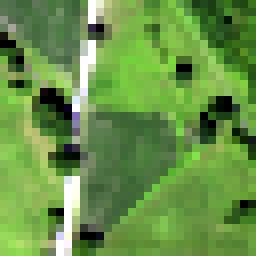
\includegraphics[trim=1cm 2cm 2cm 1cm,clip=true,width=4cm]{./figures/46_8.jpg}
\end{center}
\end{column}
\begin{column}{0.7\columnwidth}
\begin{center}
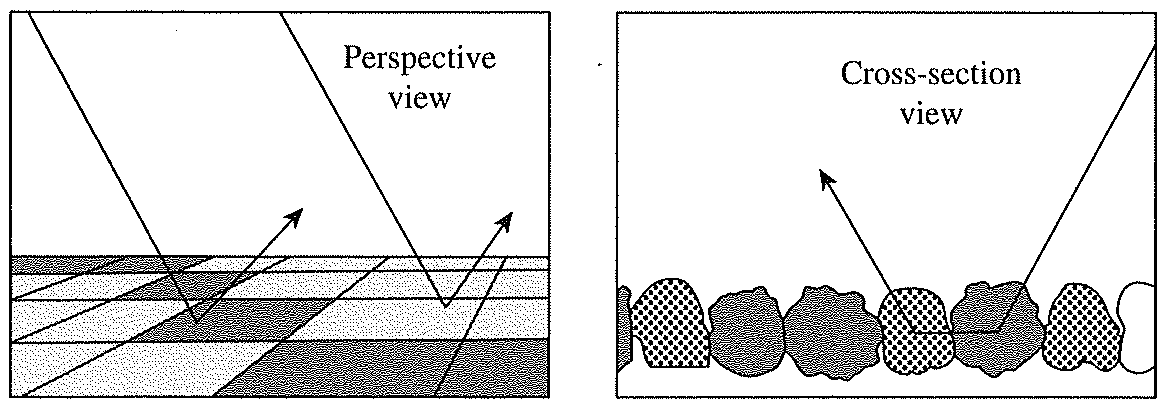
\includegraphics[width=\textwidth]{./figures/mixing_process.png}
\end{center}
\end{column}
\end{columns}
\end{frame}

\begin{frame}[label={sec:org08f0f0b}]{Example}
\begin{center}
\begin{tikzpicture}
\begin{axis}[xmin=0.4,xmax=2.5,ymin=0,ymax=1,grid,xlabel=$\lambda~({\mu}m)$,ylabel=Reflectance,width=\linewidth,height=0.9\textheight]
  \pgfplotstableread{figures/grass.txt}\loadedtable
  \addplot+[mark=none,smooth,thick,red] table[x=wave,y=grass] from \loadedtable;
  \addplot+[mark=none,smooth,thick,red!75!blue,dashed] table[x=wave,y expr=0.75*\thisrow{grass}+0.25*\thisrow{drygrass}] from \loadedtable;
  \addplot+[mark=none,smooth,thick,red!50!blue,dashed] table[x=wave,y expr=0.5*\thisrow{grass}+0.5*\thisrow{drygrass}] from \loadedtable;
  \addplot+[mark=none,smooth,thick,red!25!blue,dashed] table[x=wave,y expr=0.25*\thisrow{grass}+0.75*\thisrow{drygrass}] from \loadedtable;
  \addplot+[mark=none,smooth,thick,blue] table[x=wave,y=drygrass] from \loadedtable;
  \legend{Grass,0.75*Grass+0.25*Dry-Grass,0.5*Grass+0.5*Dry-Grass,0.25*Grass+0.75*Dry-Grass, Dry-Grass}
\end{axis}
\end{tikzpicture}
\end{center}
\end{frame}

\begin{frame}[label={sec:org51f75df}]{Applications}
\begin{itemize}
\item Conventional mapping applications \cite{Bioucas_IEEE_JSTARS_2012}:
\begin{itemize}
\item Mineral proportions
\item Vegetation covers
\end{itemize}
\item Multisource fusion:
\begin{itemize}
\item Sources of various spatial resolution
\item Sources of various spectral resolution
\end{itemize}
\item Misc:
\begin{itemize}
\item Post-improvement of classification maps
\item Clouds reconstruction of multi-temporal HI
\end{itemize}
\end{itemize}
\end{frame}

\begin{frame}[label={sec:org78f11b5}]{Unmixing processing chain}
\begin{enumerate}
\item Athmospheric correction
\item Dimensionality reduction
\item Find endmembers
\begin{itemize}
\item Hyperspectral library
\item Unsupervised
\end{itemize}
\item Find abundances
\end{enumerate}
\end{frame}
\section{Spectral mixture models}
\label{sec:org00630a2}
\subsection{Linear models}
\label{sec:org4605fb4}
\begin{frame}[label={sec:org262c3c3}]{Linear mixture model}
\begin{itemize}
\item Each pixel is a convex linear combination of endmenbers (pure spectra):
$$ \mathbf{x} = \sum_{j=1}^p\alpha_{j}\mathbf{m}_j + \mathbf{e}$$
\begin{itemize}
\item \(\mathbf{m}_j\) is the \(j^\text{th}\) endmember,
\item \(\alpha_{j}\) is the abundance of endmember \(j\),
\item \(\mathbf{e}\) is the modelling error.
\end{itemize}
\item The abundances are subject to the following constraints:
\begin{itemize}
\item Non negativity: \(\alpha_j\geq 0, \forall j=1,\ldots,p\)
\item Sum to one: \(\sum_{j=1}^p\alpha_{j}=1\).
\end{itemize}
\item Matricial formulation:
$$ \mathbf{x} = \mathbf{M}\boldsymbol{\alpha} +\mathbf{e} $$
where \(\mathbf{M}=\big[\mathbf{m}_1,\ldots,\mathbf{m}_p\big]\).
\end{itemize}
\end{frame}
\begin{frame}[label={sec:orgb6173d2}]{Geometric viewpoint}
\begin{itemize}
\item If endmembers are affinely independent, hyperspectral pixels live in
the convex hull \(C\) generated by the endmembers
\item \(C:=\Big\{\mathbf{x}=\mathbf{M}\boldsymbol{\alpha}|\sum_{j=1}^p\alpha_{j}=1,\ \alpha_j\geq 0, \forall j=1,\ldots,p \Big\}\)

\begin{center}
  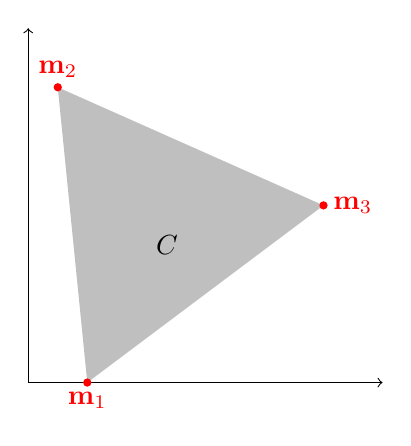
\begin{tikzpicture}[scale=1.5]
    \draw[->] (0,0) -- (3,0);
    \draw[->] (0,0) -- (0,3);
    \fill[gray!50] (0.5,0) -- (0.25,2.5) -- (2.5,1.5) -- (0.5,0);
    \draw (1,1) node[black,above right]  {$C$};
    \fill[red] (0.5,0) circle (1pt) node[below] {$\mathbf{m}_1$};
    \fill[red] (0.25,2.5) circle (1pt) node[above] {$\mathbf{m}_2$};
    \fill[red] (2.5,1.5) circle (1pt)  node[right] {$\mathbf{m}_3$};
  \end{tikzpicture}
\end{center}
\end{itemize}
\end{frame}
\subsection{Non linear model}
\label{sec:orgeafe14b}
\begin{frame}[label={sec:org032fa1a}]{Bilinear models}
\begin{itemize}
\item Consider multiple reflections \cite{6816071}
\begin{center}
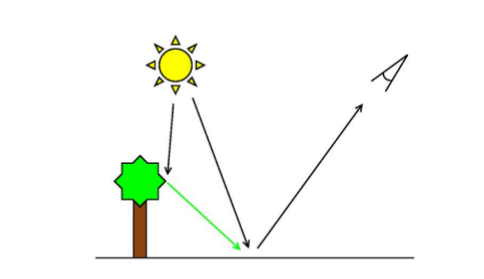
\includegraphics[width=0.5\textwidth]{./figures/fig_bilinear.png}
\end{center}
\item The model
$$\mathbf{x} = \sum_{j=1}^p\alpha_j\mathbf{m}_j + \sum_{j,k=1}^{p}\beta_{j,k}\mathbf{m}_j\odot\mathbf{m}_j$$
\item Several possible constraints on \(\alpha\) and \(\beta\)
\end{itemize}
\end{frame}
\begin{frame}[label={sec:orgb3dd81d}]{Other models}
\begin{itemize}
\item Physics based model: Intimate mixture (e.g., Hapke model)
\item Computer graphics: ray tracing
\item Kernel methods:
\begin{itemize}
\item "kernelized" linear models
\item Construct "smart" kernels
\end{itemize}
\end{itemize}
\end{frame}
\section{Subspace and Endmember extraction}
\label{sec:org55257ce}
\subsection{Subspace extraction}
\label{sec:orgfd4aa6e}
\begin{frame}[label={sec:org168f695}]{Conventional methods}
Find the subspace signal in order to search the endmembers:
\begin{itemize}
\item Principal component analysis: \emph{find the subspace that minimizes reconstruction error}
\item Minimum noise fraction: \emph{find the subspace that maximizes the SNR}
\item HySime (hyperspectral subspace identification)
\begin{itemize}
\item \emph{Estimation of the signal and noise subspaces}
\item \emph{Find the subpace that best represents the signal subspace}
\end{itemize}
\end{itemize}
\end{frame}
\subsection{Endmember extraction}
\label{sec:org1efa58a}
\begin{frame}[label={sec:org0a4c999}]{Pixel Purity Index \cite{Boardman1995}}
\begin{enumerate}
\item Apply MNF
\item Project pixels onto random vector and find \emph{extreme} projected pixels and store them
\item Pixels with the highest score are identified as the \emph{purest one}
\end{enumerate}

\begin{center}
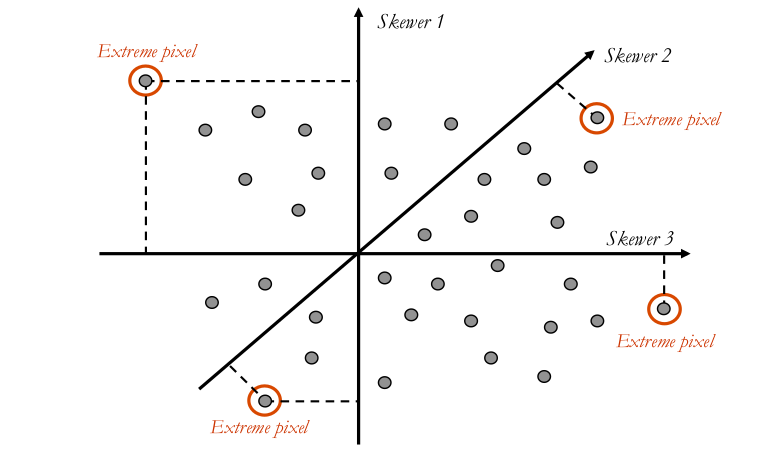
\includegraphics[width=0.6\textwidth]{./figures/ppi.png}
\end{center}
\end{frame}
\begin{frame}[label={sec:orgecb6e7f}]{N-FINDR \cite{findr}}
\begin{itemize}
\item Assumes pure pixels are present
\item Find the pixels that maximizes the volume of the simplex
\end{itemize}

\begin{center}
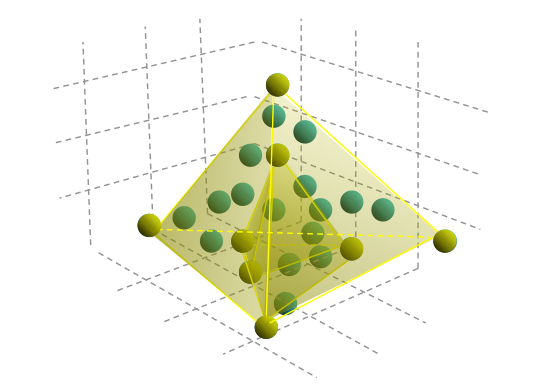
\includegraphics[width=0.6\textwidth]{./figures/nfindr.png}
\end{center}
\end{frame}
\begin{frame}[label={sec:org367bdad}]{Vertex component analysis \cite{1411995}}
\begin{itemize}
\item Iteratively project  pixels on \emph{orthogonal direction}  to the subspace
spanned by previously selected endmembers
\item New endmember correpond to the extreme of the projection
\item Works similarly to \emph{orthogonal subspace projection} but accounting for the noise
\end{itemize}
\end{frame}

\subsection{Endmember extraction in action}
\label{sec:orga48ffbc}
\begin{frame}[label={sec:orgd17fc19}]{Moffett data}
\begin{center}
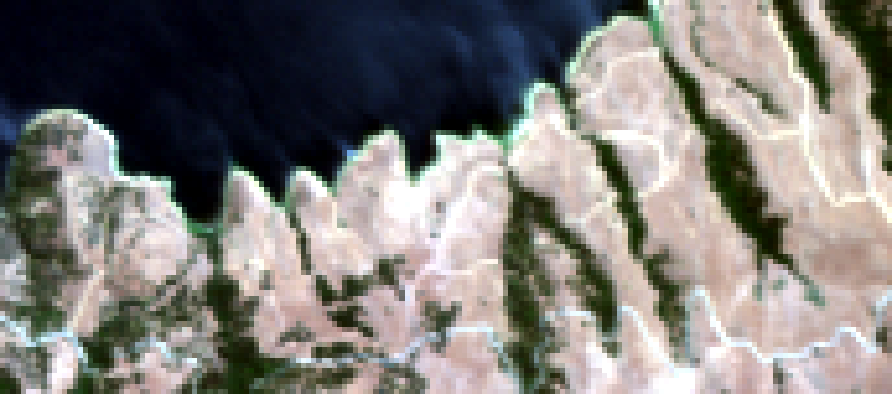
\includegraphics[width=0.7\textwidth]{./figures/moffett.png}
\end{center}
\end{frame}
\begin{frame}[label={sec:org31f66f1}]{Endmember extraction}
\begin{center}
\begin{tikzpicture}
\begin{axis}[xmin=450,xmax=2500,ymin=0,ymax=1,grid,xlabel=$\lambda~({\mu}m)$,ylabel=Reflectance,width=\linewidth,height=0.9\textheight]
  \addplot+[mark=none,smooth,thick] table[x index=0,y index=1,col sep = comma, restrict x to domain=410:1802,forget plot] {figures/endmembers.csv};
  \addplot+[mark=none,smooth,thick] table[x index=0,y index=1,col sep = comma, restrict x to domain=1952:2500] {figures/endmembers.csv};

  \addplot+[mark=none,smooth,thick] table[x index=0,y index=2,col sep = comma, restrict x to domain=410:1802,forget plot] {figures/endmembers.csv};
  \addplot+[mark=none,smooth,thick] table[x index=0,y index=2,col sep = comma, restrict x to domain=1952:2500] {figures/endmembers.csv};

  \addplot+[mark=none,smooth,thick] table[x index=0,y index=3,col sep = comma, restrict x to domain=410:1802, forget plot] {figures/endmembers.csv};
  \addplot+[mark=none,smooth,thick] table[x index=0,y index=3,col sep = comma, restrict x to domain=1952:2500] {figures/endmembers.csv};
  \end{axis}
\end{tikzpicture}
\end{center}
\end{frame}
\section{Linear unmixing}
\label{sec:org9be38b3}
\subsection{Abundance estimation}
\label{sec:org5ee5f53}
\begin{frame}[label={sec:orgb941ea6}]{Unconstrained least squares}
\begin{itemize}
\item One the  endmembers are  estimated, abundances  can be  estimated by
minimizing a reconstruction error \(Re\):
$$\hat{\boldsymbol{\alpha}}=\min_{\boldsymbol{\alpha}} \Big\{Re(\mathbf{x},\mathbf{M}\boldsymbol{\alpha})\Big\}$$

\item Conventionally \(Re\) is chosen as the mean square square error:
$$\hat{\boldsymbol{\alpha}}=\min_{\boldsymbol{\alpha}} \|\mathbf{x}-\mathbf{M}\boldsymbol{\alpha}\|^2$$

\item Without any constraint the solution is given by 
$$\hat{\boldsymbol{\alpha}} = \big(\mathbf{M}^\top\mathbf{M}\big)^{-1}\mathbf{M}^\top\mathbf{x}$$
\end{itemize}
\end{frame}
\begin{frame}[label={sec:org9e64df6}]{Constrainted least squares}
\begin{itemize}
\item Positive constraints:
\begin{eqnarray*}
  \hat{\boldsymbol{\alpha}}=\min_{\boldsymbol{\alpha}} \|\mathbf{x}-\mathbf{M}\boldsymbol{\alpha}\|^2 \\
  \text{Subject to } \alpha_j\geq 0, \forall j=1,\ldots,p
\end{eqnarray*}

\item Full set of constraints 
\begin{eqnarray*}
  \hat{\boldsymbol{\alpha}}=\min_{\boldsymbol{\alpha}} \|\mathbf{x}-\mathbf{M}\boldsymbol{\alpha}\|^2 \\
  \text{Subject to } \sum_{j=1}^p\alpha_{j}=1, \alpha_j\geq 0, \forall j=1,\ldots,p
\end{eqnarray*}
\item Not explicit solution ! Needs to optimize a quadratic function under convex constraints.
\item This is known as \emph{non negative least squares unmixing} or  \emph{fully constraints least square unmixing}
\item Easy trick: use only positive constraints that add manually the \emph{sum to one constraint} !
\end{itemize}
\end{frame}
\begin{frame}[fragile,label={sec:orgdd9c2cd}]{NNLS}
 \begin{minted}[fontsize=\footnotesize,obeytabs=true,tabsize=4,bgcolor=bg]{python}
from scipy import optimize
import scipy as sp

# Load endmembers
M = sp.loadtxt("../Unmixing/figures/endmembers.csv",delimiter=',')[:,1:]
x = 0.2*M[:,0] + 0.7*M[:,1] + 0.1*M[:,2] 

# NNLS
res = optimize.nnls(M,x)
print res[0]
\end{minted}

\begin{verbatim}
[ 0.2  0.7  0.1]
\end{verbatim}
\end{frame}

\begin{frame}[fragile,label={sec:orgbf3ed3a}]{FCLS 1/2}
 \begin{minted}[fontsize=\footnotesize,obeytabs=true,tabsize=4,bgcolor=bg]{python}
from scipy import optimize
import scipy as sp

# Loss 
def loss(alpha,x,M):
    e = x-sp.dot(M,alpha)
    return (e**2).sum()

def jac(alpha,x,M):
    e = x-sp.dot(M,alpha)
    return -2*sp.dot(M.T,e)

cons = {'type':'eq','fun':lambda alpha: 1-alpha.sum(),'jac':lambda alpha: -alpha}
bnds = ((0, None), (0, None), (0, None,))

# Load endmembers
M = sp.loadtxt("../Unmixing/figures/endmembers.csv",delimiter=',')[:,1:]
x = 0.2*M[:,0] + 0.7*M[:,1] + 0.1*M[:,2] 

# Optimize
alpha0 = sp.ones((3,))/3.0
res = optimize.minimize(loss, alpha0, args=(x,M,), jac=jac,constraints=cons, method='SLSQP',
                        bounds=bnds,)
print res['x']
\end{minted}
\begin{verbatim}
[ 0.16441937  0.67116125  0.16441937]
\end{verbatim}
\end{frame}
\begin{frame}[label={sec:orgb05cac4}]{FCLS 2/2}
\begin{center}
\begin{tikzpicture}
\begin{axis}[xmin=450,xmax=2500,ymin=0,ymax=1,grid,xlabel=$\lambda~({\mu}m)$,ylabel=Reflectance,width=\linewidth,height=0.9\textheight]
  \addplot+[mark=none,smooth,thick] table[x index=0,y index=1,col sep = comma, restrict x to domain=410:1802,forget plot] {figures/endmembers.csv};
  \addplot+[mark=none,smooth,thick] table[x index=0,y index=1,col sep = comma, restrict x to domain=1952:2500] {figures/endmembers.csv};

  \addplot+[mark=none,smooth,thick] table[x index=0,y index=2,col sep = comma, restrict x to domain=410:1802,forget plot] {figures/endmembers.csv};
  \addplot+[mark=none,smooth,thick] table[x index=0,y index=2,col sep = comma, restrict x to domain=1952:2500] {figures/endmembers.csv};

  \addplot+[mark=none,smooth,thick] table[x index=0,y index=3,col sep = comma, restrict x to domain=410:1802, forget plot] {figures/endmembers.csv};
  \addplot+[mark=none,smooth,thick] table[x index=0,y index=3,col sep = comma, restrict x to domain=1952:2500] {figures/endmembers.csv};

  \addplot+[mark=none,smooth,very thick,orange,] table[x index=0,y expr=0.2*\thisrowno{1} +0.7*\thisrowno{2} + 0.1*\thisrowno{3},col sep = comma, restrict x to domain=410:1802, forget plot] {figures/endmembers.csv};
  \addplot+[mark=none,smooth,very thick,orange,] table[x index=0,y expr=0.2*\thisrowno{1} +0.7*\thisrowno{2} + 0.1*\thisrowno{3},col sep = comma, restrict x to domain=1952:2500] {figures/endmembers.csv};
  \end{axis}
\end{tikzpicture}
\end{center}
\end{frame}
\begin{frame}[fragile,label={sec:org48a3ae1}]{Abundance maps 1/4}
 \begin{minted}[fontsize=\footnotesize,obeytabs=true,tabsize=4,bgcolor=bg]{python}
from scipy import optimize
import scipy as sp
import rasterTools as rt
import pysptools.eea as eea

# Number of endmembers
NE = 3

# Load images
im,GeoT,Proj = rt.open_data('../Data/Moffett_full.tif')
[h,w,b]=im.shape
wave = sp.loadtxt('../Data/wave_moffett.csv',delimiter=',')

# Compute endmenbers
nfindr = eea.NFINDR()
M = nfindr.extract(im.astype(float), NE, normalize=False).T

abundances = sp.empty((h,w,NE))
for h_ in xrange(h):
    for w_ in xrange(w):
        x = im[h_,w_,:]
        res = optimize.nnls(M,x)
        a = res[0]
        abundances[h_,w_,:]= (a/a.sum())

# Write the image
rt.write_data("../Data/Moffett_abundances.tif",abundances,GeoT,Proj)
\end{minted}
\end{frame}
\begin{frame}[label={sec:org8ac13c0}]{Abundances 2/4}
\begin{center}
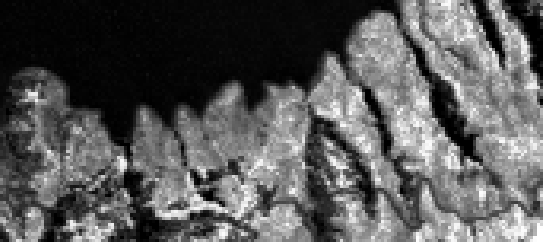
\includegraphics[width=0.7\textwidth]{./figures/abundances_baresoil.png}
\end{center}
\end{frame}

\begin{frame}[label={sec:org5b747e4}]{Abundances 3/4}
\begin{center}
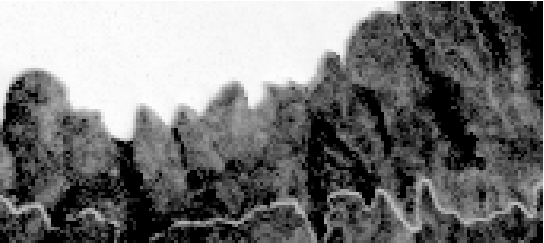
\includegraphics[width=0.7\textwidth]{./figures/abundances_water.png}
\end{center}
\end{frame}
\begin{frame}[label={sec:org8367745}]{Abundances 4/4}
\begin{center}
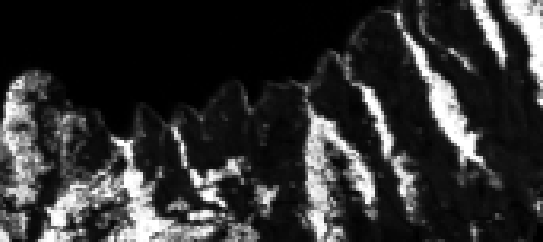
\includegraphics[width=0.7\textwidth]{./figures/abundances_vegetation.png}
\end{center}
\end{frame}
\subsection{Advances abundance estimation}
\label{sec:org6287cdc}
\begin{frame}[label={sec:org8a136af}]{Sparse unmixing}
\begin{itemize}
\item When the number of endmembers are large (e.g. selected from spectral
library), the observed  spectral vector is usually  a combination of
few ones.
\item Add \emph{sparsity} constraints in the optimization problem such as
\end{itemize}
\begin{center}
  \begin{eqnarray*}
    \min_{\boldsymbol{\alpha}} \|\boldsymbol{\alpha}\|_{0} \\
    \text{Subject to } \|\mathbf{x}-\mathbf{M}\boldsymbol{\alpha}\|^2 \leq \delta, \alpha_j\geq 0, \forall j=1,\ldots,p
  \end{eqnarray*}
\end{center}
\begin{itemize}
\item However, this problem is NP-hard: no straightforward solution
\item Use convex formulation from \emph{sparse regression} (LASSO):
\begin{center}
\begin{eqnarray*}
\min_{\boldsymbol{\alpha}} \|\mathbf{x}-\mathbf{M}\boldsymbol{\alpha}\|^2  + \lambda \|\boldsymbol{\alpha}\|_{1}\\
\text{Subject to }\alpha_j\geq 0, \forall j=1,\ldots,p
\end{eqnarray*}
\end{center}
\end{itemize}
\end{frame}
\section{References}
\label{sec:orgfe3b32b}
\begin{frame}[fragile,allowframebreaks,label=]{Bibliography}
\printbibliography
\end{frame}
\begin{frame}[label={sec:orga8bc9d5}]{}
\begin{center}
\tiny Creative Commons Attribution-ShareAlike 4.0 Unported License
\normalsize

\begin{center}

\includegraphics[width=0.1\textwidth]{figures/cc-by-sa.png}
\end{center}
\end{center}
\end{frame}
\end{document}